% This file is generated by the MATLAB m-file laprint.m. It can be included
% into LaTeX documents using the packages graphicx, color and psfrag.
% It is accompanied by a postscript file. A sample LaTeX file is:
%    \documentclass{article}\usepackage{graphicx,color,psfrag}
%    \begin{document}\input{TDwindow}\end{document}
% See http://www.mathworks.de/matlabcentral/fileexchange/loadFile.do?objectId=4638
% for recent versions of laprint.m.
%
% created by:           LaPrint version 3.16 (13.9.2004)
% created on:           23-Apr-2008 10:44:42
% eps bounding box:     15 cm x 11.25 cm
% comment:              
%

\begin{psfrags}%
\psfragscanon%
%
% text strings:
% \psfrag{x}[t][t]{\color[rgb]{0,0,0}\setlength{\tabcolsep}{0pt}\begin{tabular}{c}$x$ \end{tabular}}%

\psfrag{x}[t][t]{$x$}
\psfrag{y}[t][t]{$y(s)$}
\psfrag{a}[t][t]{$\alpha^*$}
\psfrag{u}[t][t]{$e_u(s)$}
\psfrag{v}[t][t]{$e_v(s)$}
\psfrag{t}[t][t]{$\Theta(s, x)$}
\psfrag{a}[t][t]{$\alpha^*$}
\psfrag{d}[t][t]{detector}

\psfrag{A}[t][t]{$g(s, \alpha^*)$}
%
% Figure:
\resizebox{3in}{!}{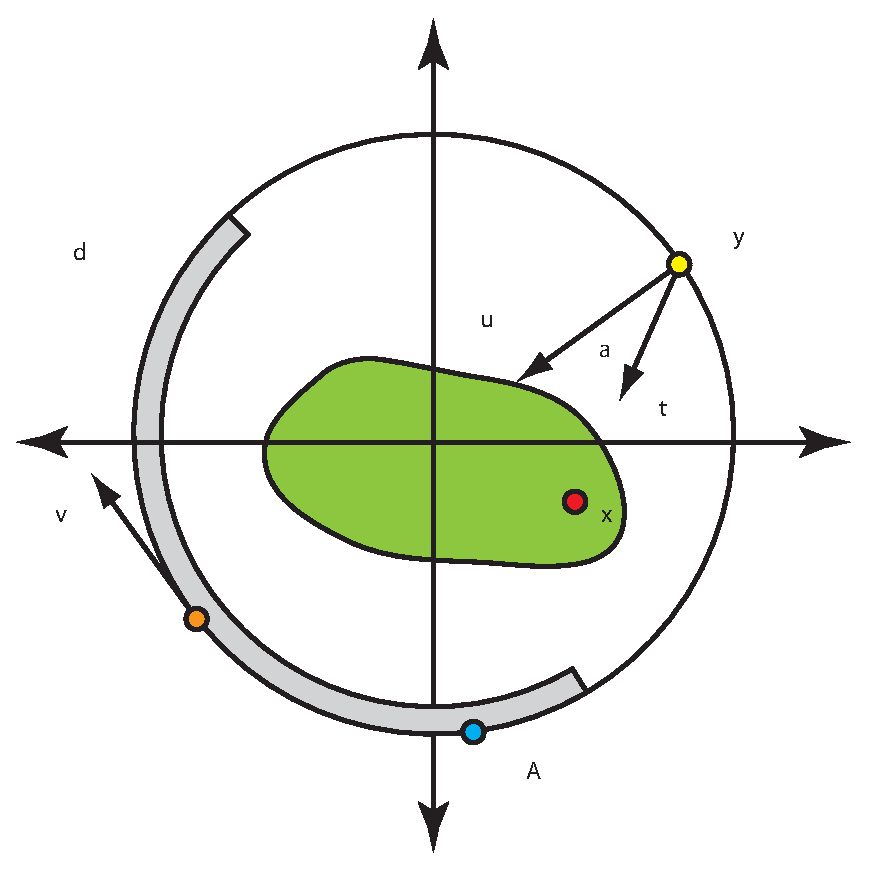
\includegraphics[width=.9\textwidth]{images/fanbeam_geometry.eps}}%
\end{psfrags}%
%
% End TDwindow.tex
